\documentclass[letterpaper]{amsart}
\usepackage{times}
\usepackage{tikz}
\usepackage{calc}
\usepackage{booktabs, siunitx}
\usepackage{graphicx}
\usetikzlibrary{arrows.meta}

\title[Homework 2]{Homework 3 \\ OR647: Queueing Theory, Spring 2021}
\author{David Prentiss}
\email{dprentis@gmu.edu}
\date{\today}

\begin{document}
\maketitle

\section{Problem 1.17} %1
Table \ref{tab:1} gives observations regarding customers at a single-server FCFS
queue.

\begin{table}
  \caption{Customer Data and Results for Problem 1.17}
  \label{tab:1}
  \begin{tabular}{SSSSSSSS}
    \toprule
    &\multicolumn{2}{c}{Data}& \multicolumn{5}{c}{Results}\\
    \cmidrule(lr){2-3}
    \cmidrule(lr){4-8}
    {Customer} & {$T^{(n)}$} & {$S^{(n)}$} & {$A^{(n)}$} & {$U^{(n)}$} & {$D^{(n)}$}
                                                         & {$W_q^{(n)}$} & {$W^{(n)}$} \\
    \midrule
    1 &   1 &   3 &    0 &    0 &    3 &    0 &   3 \\
    2 &   9 &   7 &    1 &    3 &   10 &    2 &   9 \\
    3 &   6 &   9 &   10 &   10 &   19 &    0 &   9 \\
    4 &   4 &   9 &   16 &   19 &   28 &    3 &  12 \\
    5 &   7 &  10 &   20 &   28 &   38 &    8 &  18 \\
    6 &   9 &   4 &   27 &   38 &   42 &   11 &  15 \\
    7 &   5 &   8 &   36 &   42 &   50 &    6 &  14 \\
    8 &   8 &   5 &   41 &   50 &   55 &    9 &  14 \\
    9 &   4 &   5 &   49 &   55 &   60 &    6 &  11 \\
    10 &  10 &   3 &   53 &   60 &   63 &    7 &  10 \\
    11 &   6 &   6 &   63 &   63 &   69 &    0 &   6 \\
    12 &  12 &   3 &   69 &   69 &   72 &    0 &   3 \\
    13 &   6 &   5 &   81 &   81 &   86 &    0 &   5 \\
    14 &   8 &   4 &   87 &   87 &   91 &    0 &   4 \\
    15 &   9 &   9 &   95 &   95 &  104 &    0 &   9 \\
    16 &   5 &   9 &  104 &  104 &  113 &    0 &   9 \\
    17 &   7 &   8 &  109 &  113 &  121 &    4 &  12 \\
    18 &   8 &   6 &  116 &  121 &  127 &    5 &  11 \\
    19 &   8 &   8 &  124 &  127 &  135 &    3 &  11 \\
    20 &   7 &   3 &  132 &  135 &  138 &    3 &   6 \\
    % \cmidrule(lr){3-3}
    % \cmidrule(lr){7-8}
    \midrule
    {Sum} & & 124 & & & & 67 & 191\\
    % \cmidrule(lr){3-3}
    % \cmidrule(lr){7-8}
    \midrule
    {Mean} & & 6.2 & & & & 3.35 & 9.55\\
    \bottomrule
  \end{tabular}
\end{table}
\subsection*{a}
Compute the average time in the queue and the average time in the
system.
\subsubsection*{Solution}
Let $A^{(1)}=U^{(1)}=0$. By iteratively applying the FCFS relationships to the
data, we may generate the results in Table \ref{tab:1}.
The average time in the queue and average time in the system are the averages of
their respective columns over the total number of arrivals. That is
\begin{equation*}
W_q = \frac{1}{20}\sum_{i=1}^{20}W_q^{(i)}=3.35
\end{equation*}
and
\begin{equation*}
W = \frac{1}{20}\sum_{i=1}^{20}W^{(i)}=9.55
\end{equation*}
\subsection*{b}
Calculate the average system waiting time of those customers who had
to wait for service (i.e., exclude those who were immediately taken into
service). Calculate the average length of the queue, the average number
in the system, and the fraction of idle time of the server.
What is the maximum queue length?
\subsubsection*{Solution}
From $T^{(20)}$ and $A^{(20)}$ we know that customer 21 arrives after customer
20 has left the system. Thus the system starts and ends in an empty state over
the time horizon $[A^{(0)},D^{(20)}]$ and we may apply Little's Law to find $L_q$ and $L$.
For the sample arrival rate, $\lambda=20/D^{(20)}=20/138$ we have
\begin{equation*}
L_q = \lambda W_q= \frac{20}{138}\cdot\frac{67}{20} \approx 0.486\text{ customers}
\end{equation*}
and
\begin{equation*}
L = \lambda W= \frac{20}{138}\cdot\frac{191}{20} \approx 1.384\text{ customers}
\end{equation*}

The in-service time fraction is the sum of service times divided by the length of the
time horizon. So the idle time fraction is one minus the in-service time
fraction or
\begin{equation*}
  1-\frac{1}{D^{(20)}}\sum_{i=0}^{20}S^{(i)}
  =1- \frac{124}{138}
  \approx 0.101
\end{equation*}

Finally, to find the maximum length of the queue, first note that the number of
customers in the queue can only change as a result of arrival or
service-start events.
Then calculate the number of customers in the queue $N_q(t)$ at all times $\{t\}$
such that $t$ is an arrival or service-start time. That is, for
\begin{align*}
  \{t\}&=\{0, 1, 3, 10, 16, 19, 20, 27, 28, 36, 38, 41, 42, 49, 50, 53, 55, 60, \\
  &\quad\quad 63, 69, 81, 87, 95, 104, 109, 113, 116, 121, 124, 127, 132, 135\}, \\
  \{N_q\} &= \{0, 1, 0, 0, 1, 0, 1, 2, 1, 2, 1, 2, 1, 2, 1, 2, 1, 0, 0, 0, 0, 0, 0,\\
  &\quad\quad 0, 1, 0, 1, 0, 1, 0, 1, 0\}.
\end{align*}
From which, we can see the maximum is two (2).

\section{Problem 1.18} %2
Items arrive at an initially unoccupied inspection station at a uniform rate
of one every 5 min. With the time of the first arrival set equal to 5, the
chronological times for inspection completion of the first 10 items were
observed to be 7, 17, 23, 29, 35, 38, 39, 44, 46, and 60, respectively. By
manual simulation of the operation for 60 min, using these data, develop
sample results for the mean number in system and the percentage idle time
experienced.
\subsubsection*{Solution}
From the sequences of arrival and departure times calculate the sequence of
customers in the system $\{N\}$ as before
\begin{align*}
  \{t\}&=\{0, 5, 7, 10, 15, 17, 20, 23, 25, 29, 30, 35, 38, 39, 40, 44, 45, 46, 50, 55, 60\}\\
         \{N\} &= \{0, 1, 0, 1, 2, 1, 2, 1, 2, 1, 2, 2, 1, 0, 1, 0, 1, 0, 1, 2, 2\}.
\end{align*}
Then, calculate the time interval between arrival and departure events as
\begin{equation*}
  \Delta t=\{t_{n+1}-t_{n}\} = \{5, 2, 3, 5, 2, 3, 3, 2, 4, 1, 5, 3, 1, 1, 4, 1, 1, 4, 5, 5\}
\end{equation*}

To find the mean number in the system, $L$, we integrate $N(t)$ and divide by
the length of the time horizon. That is
\begin{equation*}
  L = \frac{1}{60}\int_{\{t\}}N(t) = \frac{1}{60}\sum_{i=0}^{\|\{\Delta t\}\|}N(t_i)\Delta t_i
  =\frac{68}{60}\approx 1.133
\end{equation*}

Finally, to find the percentage idle time, we tally the length of intervals
where $N(t)= 0$. That is
\begin{equation*}
  \frac{1}{60}(5 + 3 + 1 + 1 + 4) = \frac{14}{60}\approx 0.233=\%23.3
\end{equation*}
\section{Problem 1.19} %3
Table \ref{tab:3} lists the arrival times and service durations for customers in a
FCFS single-server queue. From this data, compute $L_q$ (the time-average
number in queue) and $L_q^{(A)}$ (the average number in queue as seen by arriving
customers). For $L_q$, use a time horizon of [0, 15.27], where 15.27 is the
time that the last customer exits the system. Assume the system is empty at
$t = 0$.
\begin{table}
  \caption{Customer Data and Results for Problem 1.19}
  \label{tab:3}
  \begin{tabular}{SSSS}
    \toprule
    \multicolumn{2}{c}{Data}& \multicolumn{2}{c}{Results}\\
    \cmidrule(lr){1-2}
    \cmidrule(lr){3-4}
    {$A^{(n)}$} & {$S^{(n)}$} & {$U^{(n)}$} & {$D^{(n)}$} \\
    \midrule
    1 &  2.22 &   1.00 &   3.22 \\
    2 &  1.76 &   3.22 &   4.98 \\
    3 &  2.13 &   4.98 &   7.11 \\
    4 &  0.14 &   7.11 &   7.25 \\
    5 &  0.76 &   7.25 &   8.01 \\
    6 &  0.70 &   8.01 &   8.71 \\
    7 &  0.47 &   8.71 &   9.18 \\
    8 &  0.22 &   9.18 &   9.40 \\
    9 &  0.18 &   9.40 &   9.58 \\
    10 &  2.41 &  10.00 &  12.41 \\
    11 &  0.41 &  12.41 &  12.82 \\
    12 &  0.46 &  12.82 &  13.28 \\
    13 &  1.37 &  13.28 &  14.65 \\
    14 &  0.27 &  14.65 &  14.92 \\
    15 &  0.27 &  15.00 &  15.27 \\
    \bottomrule
  \end{tabular}
\end{table}


\subsubsection*{Solution}
From the sequences of arrival and departure times calculate the sequence of
customers in the queue $\{N_q\}$ as before
\begin{align*}
  \{t\}&=\{1, 2, 3, 3.22, 4, 4.98, 5, 6, 7, 7.11, 7.25, 8, 8.01, 8.71, 9,\\
  &\quad\quad 9.18, 9.4, 10, 11, 12, 12.41, 12.82, 13, 13.28, 14, 14.65, 15\}\\
    \{N_q\}&=\{0, 1, 2, 1, 2, 1, 2, 3, 4, 3, 2, 3, 2, 1, 2, 1, 0, 0, 1, 2, 1, 0, 1, 0, 1, 0, 0\}
\end{align*}
Then, calculate the time interval between arrival and service-start events as
\begin{align*}
  \Delta t=\{t_{n+1}-t_{n}\} = \{1, 1, 0.22, 0.78, 0.98, 0.02, 1, 1, 0.11, 0.14, 0.75, 0.01, 0.7,\\
  0.29, 0.18, 0.22, 0.6, 1, 1, 0.41, 0.41, 0.18, 0.28, 0.72, 0.65, 0.35\}
\end{align*}
To find the mean number in the queue, $L_q$, we integrate $N_q(t)$ and divide by
the length of the time horizon. That is
\begin{equation*}
  L_q = \frac{1}{15.27}\int_{\{t\}}N_q(t) = \frac{1}{15.57}\sum_{i=0}^{\|\{\Delta t\}\|}N_q(t_i)\Delta t_i
  =\frac{17.02}{15.57}\approx 1.115
\end{equation*}
To find $L_q^{(A)}$, we must first identify all customers that experienced queue
delays ($W_q{(n)}>0$). The queue length as seen by such a customer arriving at
time $t$ is $N_q(t)-1$. The average of these values is
\begin{equation*}
  L_q^{(A)} = \frac{1}{8}(1+1+1+2+3+2+1+1) = \frac{12}{8}=1.5
\end{equation*}

\section{} %4
Table \ref{tab:4a} gives the arrival and service times of a sequence of customers to
an airline ticket counter. The counter has one line and customers are served in a
first-come-first-served manner. Note: Use the same time horizon for parts (a) and
(b) in computing the average number in queue.

\begin{table}
  \caption{Customer Data and Results for Problem 4 (a)}
  \label{tab:4a}
  \begin{tabular}{SSSSS}
    \toprule
    \multicolumn{2}{c}{Data}& \multicolumn{2}{c}{Results}\\
    \cmidrule(lr){1-2}
    \cmidrule(lr){3-5}
    {$A^{(n)}$} & {$S^{(n)}$} & {$U^{(n)}$} & {$D^{(n)}$} & {$W_q^{(n)}$} \\
    \midrule
  0 &  6 &   0 &   6 &    0 \\
  6 &  4 &   6 &  10 &    0 \\
  9 &  6 &  10 &  16 &    1 \\
 10 &  1 &  16 &  17 &    6 \\
 15 &  2 &  17 &  19 &    2 \\
 17 &  1 &  19 &  20 &    2 \\
 19 &  3 &  20 &  23 &    1 \\
 23 &  5 &  23 &  28 &    0 \\
 29 &  8 &  29 &  37 &    0 \\
 35 &  6 &  37 &  43 &    2 \\
    \bottomrule
  \end{tabular}
\end{table}
\subsection*{a}
Assuming one server, compute the average wait in queue and the average
number in queue.
\subsubsection*{Solution}
See Table \ref{tab:4a}.
For the sample arrival rate, $\lambda=10/D^{(10)}=10/43$ we have
\begin{equation*}
W_q = \frac{1}{10}\sum_{i=1}^{10}W_q^{(i)}=\frac{14}{10}=1.4
\end{equation*}
and
\begin{equation*}
L_q = \lambda W_q = \frac{10}{43}\cdot\frac{14}{10} \approx 0.326
\end{equation*}
\subsection*{b}
Assuming there are two servers who are working at half speed (i.e., double
the service times), compute the average wait in queue and the average
number in queue.
Table \ref{tab:4b}
\begin{table}
  \caption{Customer Data and Results for Problem 4 (b)}
  \label{tab:4b}
  \begin{tabular}{SSSSS}
    \toprule
    \multicolumn{2}{c}{Data}& \multicolumn{2}{c}{Results}\\
    \cmidrule(lr){1-2}
    \cmidrule(lr){3-5}
    {$A^{(n)}$} & {$S^{(n)}$} & {$U^{(n)}$} & {$D^{(n)}$} & {$W_q^{(n)}$} \\
    \midrule
    0 &  12 &   0 &  12 &    0 \\
    6 &   8 &   6 &  14 &    0 \\
    9 &  12 &  12 &  24 &    3 \\
    10 &   2 &  14 &  16 &    4 \\
    15 &   4 &  16 &  20 &    1 \\
    17 &   2 &  20 &  22 &    3 \\
    19 &   6 &  22 &  28 &    3 \\
    23 &  10 &  24 &  34 &    1 \\
    29 &  16 &  29 &  45 &    0 \\
    35 &  12 &  35 &  47 &    0 \\
    \bottomrule
  \end{tabular}
\end{table}

\subsubsection*{Solution}
See Table \ref{tab:4b}.
For the sample arrival rate, $\lambda=10/D^{(10)}=10/43$ we have
\begin{equation*}
  W_q = \frac{1}{10}\sum_{i=1}^{10}W_q^{(i)}=\frac{15}{10}=1.5
\end{equation*}
and
\begin{equation*}
  L_q = \lambda W_q = \frac{10}{43}\cdot\frac{15}{10} \approx 0.349
\end{equation*}
\subsection*{c}
Compare the answers in (a) and (b) and discuss why there is a difference.
\subsubsection*{Solution}
I could not discern a significant difference between (a) and (b). I suspect this
is because in both cases, $\rho=42/43\approx 1$. At lower demand, we might
expect to see larger differences in performance.

\section{} %5
Reconstruct the Excel spreadsheet given in class for airplane arrivals
and departures to/from a single runway. Specifically, create columns containing
the following elements: Operation \#, inter-arrival time (min), actual arrival time
(min), arrival or departure (A or D), runway hold time, queue waiting time,
departure time, arrival count (1 for arrivals 0 for departures), departure count (0
for arrivals 1 for departures). The spreadsheet should also contain the following
global parameters: \% arrivals (0.5), arrival runway hold time (1 min), departure
runway hold time (1.5 min), operation arrival rate (40 / hr), average service time,
rho.
\subsection*{a}
Graph the queue-waiting time for a given sequence of 400 simulated
operations.
\subsubsection*{Solution}
See Figure \ref{fig:5a}.
\begin{figure}
  \centering
  \caption{Sample queue-waiting times for a typical scenario.
    Proportion of arrival operations = 0.5, number of operations = 400.}
  \label{fig:5a}
  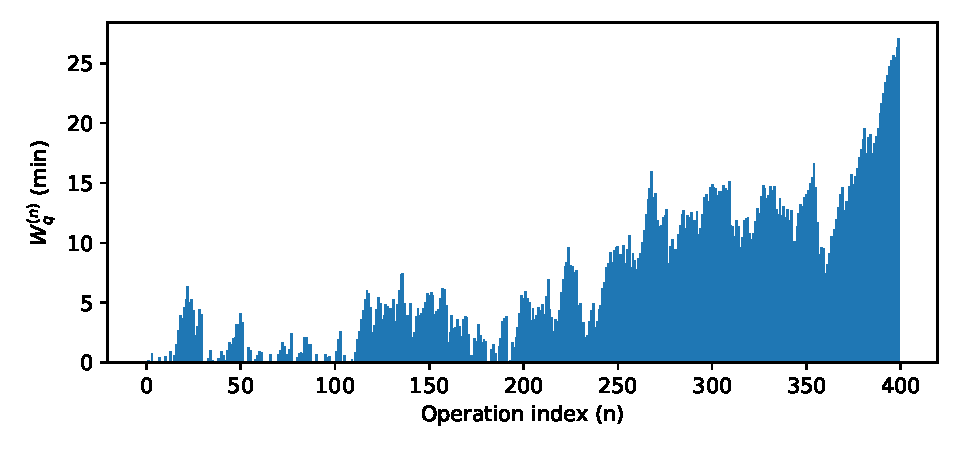
\includegraphics[width=\textwidth]{path}
\end{figure}

\subsection*{b}
Vary $\lambda$ from 5, 10, \ldots, 45, 50. Calculate the average queue-waiting time
$W_q$ for each of these cases (based on simulation of 400 operations).
\subsubsection*{Solution}
See part (c).

\subsection*{c}
Calculate the average queue-waiting time for each of these cases for an
$M/M/1$ queue with the same $\lambda$ and $\mu$. Plot both values of $W_q$ as a function
of $\lambda$ and compare the results. How good is the $M/M/1$ queue as an
approximation you’re your simulation?
\subsubsection*{Solution}
See Figures \ref{fig:5c} and \ref{fig:5cb}. Applying Little's Law to the $M/M/1$
consistently over-estimates the queue-waiting times. Relative error of the
estimate grows with $\rho$ and is impractically large as
$\rho\rightarrow 1$.
Error improves with larger numbers of operations.
The source of the error is largely the fact that service times are not exponentially
distributed, which contradicts the assumptions of the $M/M/1$ model.
Additional simulations with exponentially distributed service times with same mean
confirmed this with relative errors less than \%5 for $\rho\leq 0.8$
\begin{figure}
  \centering
  \caption{Sample average queue-waiting times by arrival rate. Boxplot shows
    summary statistics for simulations of 10000 seeds. Blue line indicates
    theoretical values from $M/M/1$ model.
    Proportion of arrival operations = 0.5, number of operations = 400.}
  \label{fig:5c}
  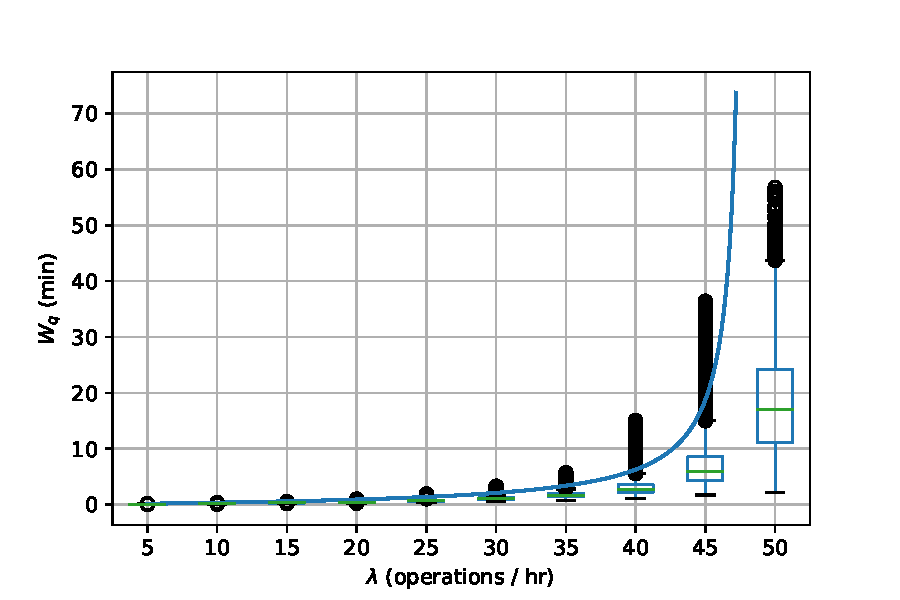
\includegraphics[width=\textwidth]{W_q1}
\end{figure}
\begin{figure}
  \centering
  \caption{Relative error by arrival rate.
    Proportion of arrival operations = 0.5, number of operations = 400.}
  \label{fig:5cb}
  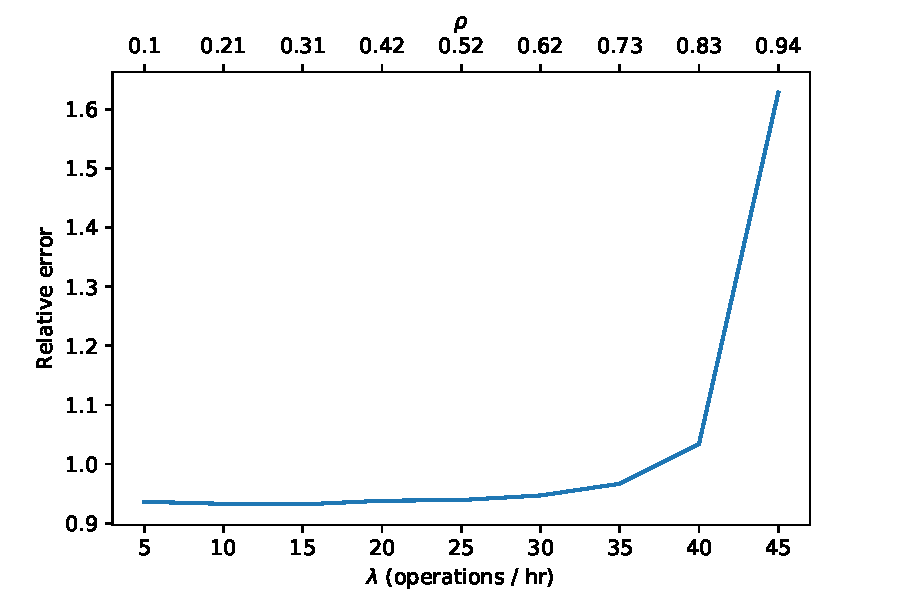
\includegraphics[width=\textwidth]{er1}
\end{figure}


\subsection*{d}
Repeat part (b) when 75\% of operations are departures.
\subsubsection*{Solution}
See Figures \ref{fig:5d} and \ref{fig:5db}.
No significant difference was noted for scenarios with a higher proportion of
departure events. This may be because arrival rates have an even lower variance
than the case with equal numbers of arrival and departure events.
non-exponentially distributed arrival times was confirmed as the most
significant source of error for this case as well.
\begin{figure}[h!]
  \centering
  \caption{Sample average queue-waiting times by arrival rate. Boxplot shows
    summary statistics for simulations of 10000 seeds. Blue line indicates
    theoretical values from $M/M/1$ model.
    Proportion of arrival operations = 0.25, number of operations = 400.}
  \label{fig:5d}
  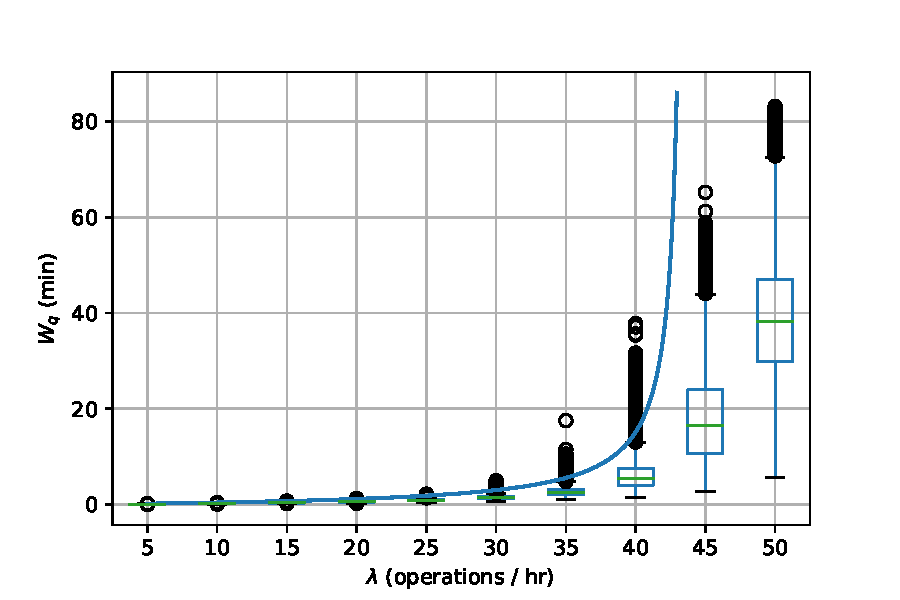
\includegraphics[width=\textwidth]{W_q2}
\end{figure}
\begin{figure}
  \centering
  \caption{Relative error by arrival rate.
    Proportion of arrival operations = 0.25, number of operations = 400.}
  \label{fig:5db}
  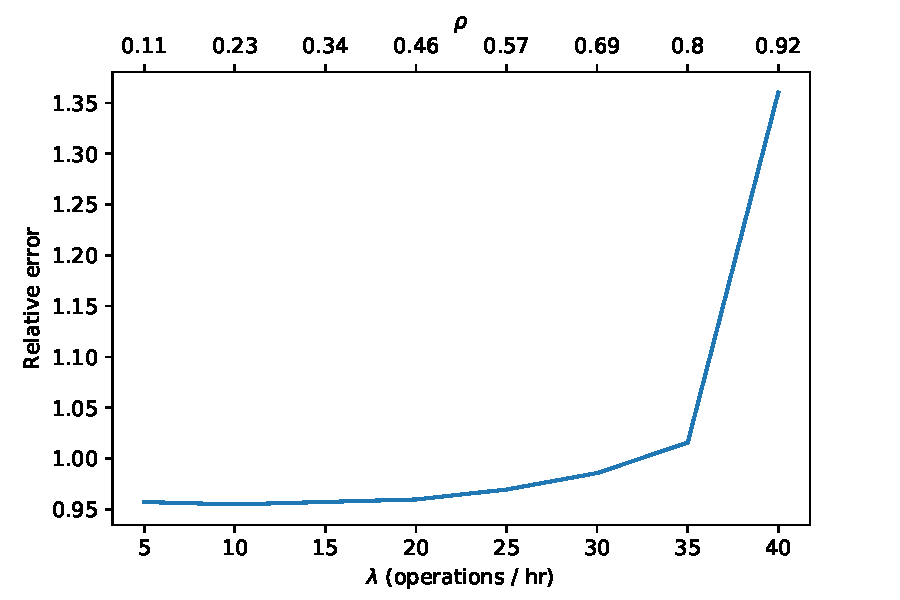
\includegraphics[width=\textwidth]{er2}
\end{figure}


\section{} %6
A hardware store has a ``merchandise pickup'' window where customers arrive to
load previously purchased items into their car. Arrivals to the pickup window
follow a Poisson process with rate 45 per hour. The time for a store employee to
load merchandise into a customer’s car is exponentially distributed with a mean of
3 minutes. There are 3 employees. What is the average time it takes for a
customer to get his/her merchandise loaded into the car (wait in queue plus
service time)?
\subsubsection*{Solution}
Let $\lambda = \frac{45}{60} = 0.75$, $\mu=\frac{1}{3}$,
and $c=3$. Then $r=\frac{\lambda}{\mu}=\frac{9}{4}=2.25$ and $\rho = \frac{r}{c} = \frac{2.25}{3} = 0.75$.
For an $M/M/c$
\begin{equation*}
  p_0=\left( \frac{r^c}{c!(1-\rho)}+\sum_{n=0}^{c-1}\frac{r^n}{n!}\right)^{-1}\approx 0.075
\end{equation*}
So
\begin{equation*}
  L_q=\left( \frac{r^c\rho}{c!(1-\rho)^2}\right)p_0
  =\left( \frac{(2.25)^5(0.75)}{3!(1-(0.75))^2}\right)0.075\approx 1.703\text{ customers}
\end{equation*}
and then
\begin{equation*}
  W = \frac{1}{\mu}+\frac{L_q}{\lambda}
  =\frac{1}{1/3}+\frac{1.703}{0.75}
  \approx 5.271\text{ minutes}
\end{equation*}

\section{} %7
A local polling location has 5 voting machines. People arrive to cast their votes
according to a Poisson process with rate $\lambda=75$ per hour. The time to cast a ballot
is exponential with a mean of 2 minutes.
\subsection*{a}
What is the fraction of time that a given voting machine is being utilized?
\subsubsection*{Solution}
Let $\lambda = \frac{75}{60} = 1.25$, $\mu=\frac{1}{2}=0.5$,
and $c=5$. Then $r=\frac{\lambda}{\mu}=\frac{1.25}{0.5}=2.5$
The long-term average fraction of occupied server time for an $M/M/c$ is $\rho = \frac{r}{c} = \frac{2.5}{5} = 0.5$.
\subsection*{b}
What is the fraction of time that 3 or fewer machines are in use?
\subsubsection*{Solution}
The fraction of time that 3 or fewer machines are in use is the sum of the
probabilities $p_n$ that
the system is in state $n$ where $n\leq3$ or
\begin{equation*}
  \text{Pr}\{n\leq3\}=\sum_{n=0}^3p_n=\sum_{n=0}^3\frac{\lambda^n}{n!\mu^n}p_0
\end{equation*}
For the $M/M/c$ model
\begin{equation*}
  p_0=\left( \frac{r^c}{c!(1-\rho)}+\sum_{n=0}^{c-1}\frac{r^n}{n!}\right)^{-1}\approx 0.080
\end{equation*}
and
\begin{equation*}
  \text{Pr}\{n\leq3\}
  = 0.080\cdot\sum_{n=0}^3\frac{(1.25)^n}{n!(0.5)^n}
  \approx 0.739
\end{equation*}
\subsection*{c}
What is the average line length?
\subsubsection*{Solution}
\begin{equation*}
  L_q=\left( \frac{r^c\rho}{c!(1-\rho)^2}\right)p_0
  =\left( \frac{(2.5)^5(0.5)}{5!(1-(0.5))^2}\right)0.080\approx 0.130\text{ customers}
\end{equation*}

\section{} %8
Arrivals to a queueing system follow a Poisson process with rate 18 per hour.
Service times are exponential with rate 20 per hour. Each server is paid \$40 per
hour while working and \$10 per hour while idle. The company determines that it
loses \$2 per customer per hour spent waiting in the queue, due to ``ill-will'' or lost
customer loyalty.
\subsection*{a}
What is the hourly cost to the company if 1 server is employed?
\subsubsection*{Solution}
Let $\lambda = 18$, $\mu=20$,
and $c=1$. Then $r=\frac{\lambda}{\mu}=\frac{18}{20}=0.9$ and
$\rho = \frac{r}{c} = \frac{0.9}{1} = 0.9$.
If there is a single server, we may adopt the $M/M/1$ model and
$L_q=\frac{\rho^2}{(1-\rho)}=\frac{0.9^2}{1-0.9}=8.1$.
The cost of the system then is
\begin{equation*}
  \$40\cdot r + \$10(c-r) + \$2\cdot L_q
  =\$40\cdot 0.9 + \$10(1-0.9) + \$2\cdot 8.1
  = \$53.20\text{ per hour}
\end{equation*}
\subsection*{b}
What is the hourly cost to the company if 2 servers are employed?
\subsubsection*{Solution}
Let $\lambda = 18$ and $\mu=20$ as before,
and $c=2$. Then $r=\frac{\lambda}{\mu}=\frac{18}{20}=0.9$ as before and
$\rho = \frac{r}{c} = \frac{0.9}{2} = 0.45$.
Since there are two servers, we chose the $M/M/c$ model where
\begin{equation*}
  p_0=\left( \frac{r^c}{c!(1-\rho)}+\sum_{n=0}^{c-1}\frac{r^n}{n!}\right)^{-1}\approx 0.379
\end{equation*}
and then
\begin{equation*}
  L_q=\left( \frac{r^c\rho}{c!(1-\rho)^2}\right)p_0\approx 0.229
\end{equation*}
The cost then is
\begin{equation*}
  \$40\cdot r + \$10(c-r) + \$2\cdot L_q
  =\$40\cdot 0.9 + \$10(2-0.9) + \$2\cdot 0.012
  \approx \$47.46\text{ per hour}
\end{equation*}

\subsection*{c}
If the company adds a 3rd server, would the cost go up or down compared
with 2 servers? (Give a one- or two-sentence explanation without working
the numbers out fully).
\subsubsection*{Solution}
Adding a third server would likely increase the cost as compared with two
servers since, in the later case, the cost of the queue is only \$0.46 per hour,
whereas the cost of an additional server is at least \$10 per hour.
We know that such a break-even point for additional servers exists since the
cost of ``ill will'' is bound below at zero, but the cost of idle employees is
positive and unbound above.

\section{Problem 3.32} %9
You are managing a call center where the arrival rate is 500 calls per hour
and the service time is exponential with a mean of 2 minutes.
\subsection*{a}
What is the approximate number of servers needed so that the probability that a
customer has a non-zero wait in queue is 10\%?

\subsubsection*{Solution}
Let $\lambda = \frac{500}{60}=\frac{25}{3}$, $\mu=\frac{1}{2}=0.5$, and $\alpha=0.10$. Then
$r=\frac{\lambda}{\mu}=\frac{50}{3}$, $\beta\approx1.420$ and
\begin{equation*}
  c\approx r + \beta\sqrt{r} = 22.465 \approx 23
\end{equation*}

\subsection*{b}
If the arrival rate increases by 60\%, what is the approximate number of
servers needed to maintain the same level of service?

\subsubsection*{Solution}
Let $\lambda = 1.6\cdot\frac{500}{60}=\frac{40}{3}$, $\mu=\frac{1}{2}=0.5$,
and $\beta\approx1.420$. Then $r=\frac{\lambda}{\mu}=\frac{80}{3}$ and
\begin{equation*}
  c\approx r + \beta\sqrt{r} = 34.000 \approx 34
\end{equation*}

\subsection*{c}
If the average time to complete a call increases by 1 minute (assuming
the original arrival rate of 500 calls per hour), what is the approximate
number of servers needed to maintain the same level of service?
\subsubsection*{Solution}
Let $\lambda = \frac{500}{60}=\frac{25}{3}$, $\mu=\frac{1}{3}$
and $\beta\approx1.420$. Then $r=\frac{\lambda}{\mu}=25$ and
\begin{equation*}
  c\approx r + \beta\sqrt{r} = 32.101 \approx 33
\end{equation*}

\subsection*{d}
For parts (a) and (b), compute the exact minimum number of servers
needed to achieve no more than 10\% probability of non-zero wait in
queue. Compute the exact expected wait in queue for the two scenarios.
Are they the same?
\subsubsection*{Solution}
For part (a) Let $r=\frac{\lambda}{\mu}=\frac{50}{3}$. Then $\rho=r/c = \frac{50}{3c}$.
The probability of nonzero wait time is given by
\begin{equation*}
  C(c,r)=\frac{r^c}{c!(1-\rho)}\left( \frac{r^c}{c!(1-\rho)}+\sum_{n=0}^{c-1}\frac{r^n}{n!}\right)^{-1}
\end{equation*}
Starting with our estimate, $c\approx23$, we have
\begin{align*}
  C(23,\frac{50}{3}) &= 0.101 > 0.10 \\
  C(24,\frac{50}{3}) &= 0.064 < 0.10\ \checkmark
\end{align*}

For part (b) Let $r=\frac{\lambda}{\mu}=\frac{80}{3}$ with $C(c,r)$ as before.
Starting with our estimate, $c\approx34$, we have
\begin{align*}
  C(34,\frac{80}{3}) &= 0.122 > 0.10 \\
  C(35,\frac{80}{3}) &= 0.085 < 0.10\ \checkmark
\end{align*}

\section{Problem 3.37} %10
You are managing a call center where arrivals follow a Poisson process with
rate of 300 calls per hour and the service time is exponential with a mean of
2 minutes.
\subsection*{a}
What is the approximate number of servers needed so that the probability that a
customer has a nonzero wait in queue is 5\%?

\subsubsection*{Solution}
Let $\lambda = \frac{300}{60}=5$, $\mu=\frac{1}{2}=0.5$, and $\alpha=0.05$. Then
$r=\frac{\lambda}{\mu}=10$, $\beta\approx1.740$ and
\begin{equation*}
  c\approx r + \beta\sqrt{r} = 15.502 \approx 16
\end{equation*}

\subsection*{b}
If the arrival rate doubles, what is the approximate number of servers
needed to maintain the same level of service?

\subsubsection*{Solution}
Let $\lambda = 2\cdot\frac{300}{60}=10$, $\mu=\frac{1}{2}=0.5$, and $\beta\approx1.740$. Then
$r=\frac{\lambda}{\mu}=20$ and
\begin{equation*}
  c\approx r + \beta\sqrt{r} = 27.781 \approx 28
\end{equation*}

\subsection*{c}
Suppose that you are given the steady-state probabilities $p_0,p_1,\ldots,p_n$.
Give a formula or procedure for computing the expected number of
customers in queue and the variance of the number of customers in
queue using these values.

\subsubsection*{Solution}
Given a sequence of $n+1$ steady-state probabilities with $n$ large enough that
$p_n \approx 0$, the average number in the queue, $L_q$, is approximated by the
sums of the length of the queue in each state weighted by the probability of its
respective probability or


\begin{equation*}
  L_q = \sum_{i=c+1}^n(i-c)p_i
\end{equation*}
where $c$ is the number of servers.
Here, $i-c$ serves as the size of the queue in each state $n$ and, we may ignore
$i\leq c$ since the length of the queue in those states is 0.
The variance then is
\begin{equation*}
  \sigma_{L_q}^2 = \sum_{i=c+1}^n(i-c-L_q)^2p_i
\end{equation*}
Care must be taken with an estimate such as this since the distribution of queue
lengths may be heavy-tailed.
As such, $n$ may need to be very large to avoid a significant estimation error.

\end{document}
